
%%%%%%%%%%%%%%%%%%%%%%%%%%%%%%%%%%%%%%%%%%%%%%%%%%%%%%%%%%%%%%%%
% neměnit
%
\documentclass[a4paper,10pt,twocolumn]{article}
\usepackage{lmodern}
\usepackage[czech]{babel}
\usepackage[T1]{fontenc}
\usepackage[utf8]{inputenc}
\usepackage{graphicx}
\usepackage{float}
\usepackage[top=0.5cm,bottom=2cm,left=1cm,right=1cm]{geometry}
%
%%%%%%%%%%%%%%%%%%%%%%%%%%%%%%%%%%%%%%%%%%%%%%%%%%%%%%%%%%%%%%%%


%%%%%%%%%%%%%%%%%%%%%%%%%%%%%%%%%%%%%%%%%%%%%%%%%%%%%%%%%%%%%%%%
% dopište jméno článku,který aplikujete, svá jména, školní(!!!) emaily (emaiy jakol milasek328@seznam.cz apod. prosím ne...)
%
\title{Technická zpráva k semestrální práci z předmětu MI-ROZ \\ Identifikaca duhovek pomocí algoritmu SIFT}
\date{\today}
\author{Zdeněk Svatoň\\ svatozde@fit.cvut.cz}
%
%%%%%%%%%%%%%%%%%%%%%%%%%%%%%%%%%%%%%%%%%%%%%%%%%%%%%%%%%%%%%%%%


%%%%%%%%%%%%%%%%%%%%%%%%%%%%   TEXT   %%%%%%%%%%%%%%%%%%%%%%%%%%%%%%%%%%%%
%
%
\begin{document}
\maketitle
\begin{abstract}
Práce zabývá možností využití algoritmu SIFT pro identifikaci duhovek, zároveň vyběrem vhodného předzpracování a následné práci s detekovanými příznaky obrazků duhovek.
\end{abstract}

%%%%%%%%%%%%%%%%%%%%%%%%%%   SEGMENTER   %%%%%%%%%%%%%%%%%%%%%%%%%%%%%%%%%%%
%
\section{Porovnávání}

Jak bylo řečené výše hlavním algoritmem použitým v této prácí je \emph{SIFT} což je zkratka pro \emph{scale-invariant feature transform} jejímž autorem je David G. Lowe.
Loweova metoda pro generování obrazových prvků transformuje obraz do velké kolekce vektorů, z nichž každý je invariantní k převodu, škálování, rotaci obrazu a částečně invariantní ke změnám osvětlení a robustní k lokálnímu geometrickému zkreslení.
Tyto rysy sdílejí podobné vlastnosti s neurony v primární vizuální kůře, které kódují základní formy, barvu a pohyb pro detekci objektů ve vidění primátů.
Klíčová umístění jsou definována jako maxima a minima výsledku rozdílu Gaussovských funkcí aplikovaných v měřítkovém prostoru na řadu vyhlazených a převzorkovaných obrázků. Body s nízkým kontrastem jsou zahozeny.
Dominantní gradienty jsou přiřazeny lokalizovaným klíčovým bodům. Tyto kroky zajišťují, že klíčové body jsou stabilnější pro přiřazování a rozpoznávání.

Dalším faktem je že v úloze byly použity normalizvované obrázky duhovek, bylo tedy možní vzít v úvahu i pozici exporotvaných deskriptorů a shodné deskriptory které byly na příliš rozdílných pozicích bylo možné zanedbat.
K výpočtu této vzdáoenosti byla požita standarní euklidovská vzdálenost.

\subsection{Příklad:}  Na obrázku dole je vidět "dobrý" diky velkému množství příznaků odfiltrovaných díky relativně velkému prahu pro vzdálenost mezi deskriptory a poté dalšímu filtrování které vylučí keypointy s příliš rozdílnými pozicemi zbyde typicky cca 15 dobrých porovnání.
Pokud jde o jinou zorničku počet těchto keypointu je mezi 0-5.


\begin{figure}[H]
       \begin{center}
              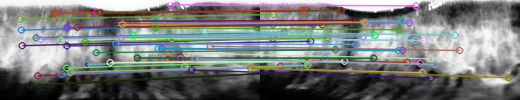
\includegraphics[width=6cm]{imgs/example_match.png}
       \end{center}
       \caption{Ukázka výsledku porovnávání dvou rozdílných obrázku identických
       duhovek. Vsimňete si především podobné pozice a rozmístění klíčových bodů.}
       \label{fig3}
\end{figure}

Dále si všiměte že původní obrázky byly ořéznuty. Především zprava a zleva kde se obvykle vyskytovaly takzvané světelné bloby a často i řasy které do obrázku vnášeli příliš mnoho podobných descriptorů, což vedklo k časté chybě druhého typu.

\begin{figure}[H]
    \begin{center}
        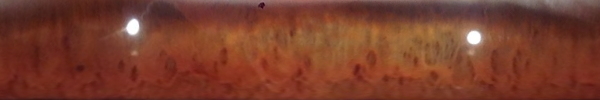
\includegraphics[width=6cm]{imgs/original_with_blobs.png}
    \end{center}
    \caption{Příklda původního obrázku.}
    \label{fig3}
\end{figure}

\begin{figure}[H]
    \begin{center}
        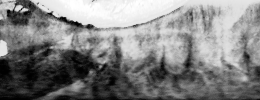
\includegraphics[width=6cm]{imgs/croped.png}
    \end{center}
    \caption{Příklda oříznutého předzpracovaného obrázku.}
    \label{fig3}
\end{figure}

%==================================    příznaky   ==================================================

\subsection{Příznaky}

Metoda SIFT využívá klasickkou kombinaci descriptor a jejich pozic tzv. keypoints.

\begin{figure}[H]
      \begin{center}
            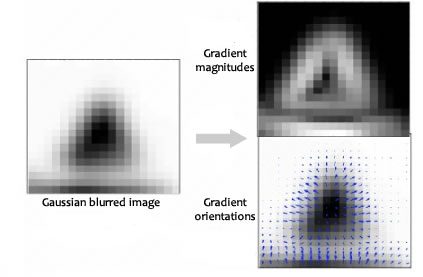
\includegraphics[width=6cm]{imgs/sift-orientation-window.jpg}
      \end{center}
      \caption{Ukázka SIFT descriptoru.}
\end{figure}

%==================================    postprocessing   ===============================================



%%%%%%%%%%%%%%%%%%%%%%%%%%   VÝSLEDKY   %%%%%%%%%%%%%%%%%%%%%%%%%%%%%%%%%%%
%
\section{Výsledky}

\begin{description}
    \item[$\bullet$ Počet obrázků]  813
    \item[$\bullet$ Počet tříd] 150 (Pravé a levé oko jsou různe třídy)
\end{description}

\begin{center}
    \begin{tabular}{||c c||}
        \hline
        Počet testovacích obrázků  & Úspěšnost klasifikace\\ [0.5ex]
        \hline\hline
        25 & 84\% \\
        \hline
        85 & 81\% \\
        \hline
        255 & 77\% \\
        \hline
        400 & 64\% \\
        \hline
        \hline
    \end{tabular}
\end{center}



%Vejde-li se to do zprávy, uveďte i hodnoty CS vaší implementace. 

%%%%%%%%%%%%%%%%%%%%%%%%%%   Možnosti vylepšení   %%%%%%%%%%%%%%%%%%%%%%%%%%%%%%%%%%%
%
\subsection{ Možnosti vylepšení}

\begin{description}
    \item[$\bullet$ BOF]  vyoužitím implementace bag of features z Opencv by se podstaně zrychlila klasifikace, nicméně jsem převědčen že by to mělo negativní vliv na úspěšnost.
    \item[$\bullet$ Využití všech tří kanálů] toto by jistě přispělo k uspěšnosti klasifikace, nicméně čas běhu by se ztrojnásobil. Proto jsem od tohoto řešení upustil
    \item[$\bullet$ Rozmístění deskcriptorů] V mé práci jsem uvažoval jen polohu jednotlivých deskriptorů nikoli jejich rozmístění. Přemýšlel jsem o zkonstruování trojúhelníkových mřížek v obou obrazcích, a jejich porovnání. Bohužel jsem nenašel žádný už implementovaný algoritmus, který bych mohl využit.
\end{description}

%%%%%%%%%%%%%%%%%%%%%%%%%%   SHRNUTÍ   %%%%%%%%%%%%%%%%%%%%%%%%%%%%%%%%%%%
%
\section{Shrnutí}

Metoda se ukázála i na relativně nekvalitních datech jako celkem úspěšná, ovšem uspěšnost klasifikace rychle klesala se snižujícím se počtem trénovacích (známých) obrazků.
Nicméně největší problém pro jakékoli praktické využití je extrémně nízká rychlost.
Bez využití nějakého jiného klasifikátoru, je celkem pomalá i na malám datasetu, porovnání testovaného obrázku se všemi třídami trvá přes minutu.
I s použití paralelizace na téměř všech jádrech (v mém případě 12-1).
%
%%%%%%%%%%%%%%%%%%%%%%%%%%%%%%%%%%%%%%%%%%%%%%%%%%%%%%%%%%%%%%%%%%%


%%%%%%%%%%%%%%%%%%%%%%%%%%%   REFERENCE   %%%%%%%%%%%%%%%%%%%%%%%%%%%%%%%%%
%
\bibliographystyle{unsrt}
\bibliography{roz}
%
%%%%%%%%%%%%%%%%%%%%%%%%%%   END OF TEXT   %%%%%%%%%%%%%%%%%%%%%%%%%%%%%%%%%%

%%%%%%%%%%%%%%%%%%%%%%%%%%   INFO   %%%%%%%%%%%%%%%%%%%%%%%%%%%%%%%%%%%%%
% celou tuto sekci ve vaší práci vynechejte
%
\vspace{-2mm}
\begin{center}
\line(1,0){250}
\end{center}
\vspace{-2mm}



\end{document}
